\documentclass{standalone}
\usepackage{tikz}
\usepackage{pgfplots}

\begin{document}
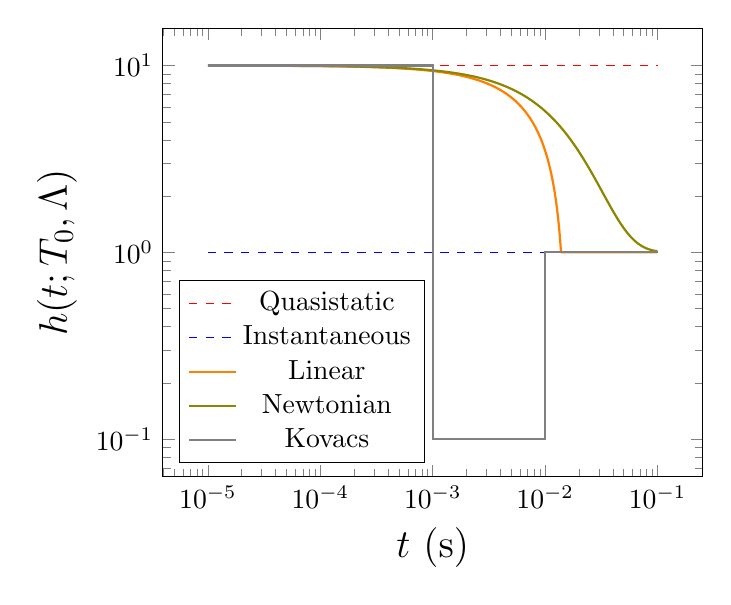
\begin{tikzpicture}
    \begin{loglogaxis}[xlabel=\Large{$t$ (s)}, ylabel=\Large{$h(t;T_0,\Lambda)$}, legend pos=south west]
        \addplot[dashed, red, domain=1e-5:1e-1, samples=5]{10};
        \addlegendentry{Quasistatic};
        \addplot[dashed, blue, domain=1e-5:1e-1, samples=5]{1};
        \addlegendentry{Instantaneous};
        \addplot[thick, domain=1e-5:1e-1, samples=500, orange]{max(10*(1-65*x), 1)};
        \addlegendentry{Linear}
        \addplot[thick, domain=1e-5:1e-1, samples=500, olive]{9*exp(-65*x)+1};
        \addlegendentry{Newtonian}
        \addplot[thick, gray] coordinates{(1e-5,10) (1e-3, 10) (1e-3,0.1) (1e-2,0.1) (1e-2,1) (1e-1,1)};
        \addlegendentry{Kovacs}
    \end{loglogaxis}
\end{tikzpicture}
\end{document}